%equations, bib. \\

%Should I state that regressors, coefficients etc are all names that mean the regression coefficients?
%Am I allowed to use words as thesis and paper for this project? E.g "in this paper..."

\section{Linear regression models}
In the following section we will follow the derivations and results of \citet{GLMM_book} and \citet{GLMM_book_old}, however the book might have used scalar notation.
\subsection{Multiple linear regression}
Linear regression aims to model the relationship between a response $y_i, i\in\{1, 2, ..., n\}$ and covariates $\mathbf{x}_i$, where $\mathbf{x}_i = (x_{i, 1}, x_{i, 2}, ..., x_{i, p})$, by estimating the regression coefficients $\boldsymbol{\beta} = (\beta_0, \beta_1, ..., \beta_p)$. The linear regression can be written in matrix form as
\begin{equation}
    \label{eq:lin_reg}
    \mathbf{y} = \mathbf{X}\boldsymbol{\beta} + \boldsymbol{\varepsilon} \ , 
\end{equation}
where $\boldsymbol{\varepsilon}=(\varepsilon_1, \varepsilon_2, ..., \varepsilon_n)$ is the random error term. It is assumed that the response is independent, and the error term is independent and identically distributed(iid) following a normal distribution with mean zero and variance $\sigma^2$, \textit{i.e.} $\varepsilon_i \sim \mathcal{N}(0, \sigma^2)$. 
By inspection one can state that, given the covariates $\mathbf{X}$, 
\begin{equation}
    \begin{split}
        \mathbb{E}(\mathbf{y} \lvert \mathbf{X}) = \mathbb{E}(\mathbf{X}\boldsymbol{\beta} + \boldsymbol{\varepsilon}) = \mathbf{X}\boldsymbol{\beta} \ ,  \\
        \text{Var}(\mathbf{y} \lvert \mathbf{X}) = \text{Var}(\mathbf{X}\boldsymbol{\beta}) + \text{Var}(\boldsymbol{\varepsilon}) = \text{Var}(\boldsymbol{\varepsilon}) = \sigma^2\mathbf{I} \ ,
    \end{split}
\end{equation}
where $\mathbf{I} \in \mathbb{R}^{n \times n}$ is the identity matrix. 
It is then straightforward to see that $\mathbf{y}$ follows the conditional normal distribution
\begin{equation}
    \mathbf{y} \lvert \mathbf{X} \sim \mathcal{N}_n(\mathbf{X}\boldsymbol{\beta}, \sigma^2 \mathbf{I})
\end{equation}
and from this distribution of $\mathbf{y}$ it can be shown that the likelihood function is expressed as
\begin{equation}
    \mathcal{L}(\boldsymbol{\beta}, \sigma^2 \lvert \mathbf{y}) \propto \sigma^{-n/2}\exp\left(-\frac{1}{2\sigma^2}(\mathbf{y}-\mathbf{X}\boldsymbol{\beta})^T(\mathbf{y}-\mathbf{X}\boldsymbol{\beta})\right)
\end{equation}
and that the maximum likelihood estimator (MLE) of $\boldsymbol{\beta}$, which maximizes the likelihood, is given by
\begin{equation}
    \label{eq:beta_hat}
    \hat{\boldsymbol{\beta}} = (\mathbf{X}^T\mathbf{X})^{-1}\mathbf{X}^T\mathbf{y} \ .
\end{equation}

\subsection{Linear mixed models (LMM's)}
\label{sec:LMM}
Data often comes in clustered form, for example due to repeated measurements of the covariate over time. 
Clustered data violate with the assumption of independent responses in linear regression and must be properly accounted for. One solution to this is to introduce random effects that are cluster specific, but independent of the fixed effects and the other clusters. Let the population contain $m$ underlying clusters, with $n_j\ , j=1, ..., m$ observations in each cluster, so that $\mathbf{y} \in \mathbb{R}^{(N \times 1)}$ where $N = \sum_{j=1}^m n_j $. Assume that we investigate $q$ random effects, including a random intercept and $q-1$ random slopes, such that the random effects vector can be written as 
\begin{equation}
    \label{eq:alpha}
    \boldsymbol{\alpha} = (\boldsymbol{\alpha}_1, ..., \boldsymbol{\alpha}_{m})^T \ ,
\end{equation}
where each $\boldsymbol{\alpha}_j \in \mathbb{R}^{q \times 1}$ is assumed independent and represents the random effects for cluster $j$ and has length $q$. For a cluster $j$ the vector $\boldsymbol{\alpha}_j \sim \mathcal{N}_q(\mathbf{0}, \mathbf{Q})$ where $\mathbf{Q}$ is the $q \times q$ unknown covariance for the random effects, assumed to be positive definite. 
If the random effects for each cluster are independent of each other, the covariance matrix $\mathbf{Q} = \text{diag}(\tau_0^2, ..., \tau_q^2)$.
The linear mixed model now takes the form
\begin{equation} \label{eq:LMM}
    \mathbf{y} = \mathbf{X}\boldsymbol{\beta} + \mathbf{U}\boldsymbol{\alpha} + \boldsymbol{\varepsilon} \ ,
\end{equation}
where $\mathbf{X} \in \mathbb{R}^{N \times p}$ is the design matrix for the fixed effects, $\boldsymbol{\beta} \in \mathbb{R}^{p \times 1}$ are the regression coefficients for the fixed effects, $\mathbf{U} = \text{diag}(\mathbf{U_j}) \ , \in \mathbb{R}^{N \times q}$ is the design matrix for the random effects and $\mathbf{U}_j \in \mathbb{R}^{n_j \times q}$ is the design matrix for cluster $j$. 
Since $\boldsymbol{\alpha}$ is a random variable, the parameter to estimate is the variance of each random effect $\mathbf{Q}_{kk}=\tau_k^2$ and their covariance $\mathbf{Q}_{k, l} = \tau_{k, l}$, where $k, l =1, ..., q$. 
In this model the independence between clusters are conserved for the response as a whole, but it expresses the correlation that observations of the same cluster have through the random effects.
As for the simple linear regression it is assumed that $\mathbf{X}\boldsymbol{\beta}$ is fixed, and that $\mathbf{U}$ is given, so they do not contribute to the model's variance. Therefore, the conditional expectation $\mathbb{E}(\mathbf{y} \lvert \mathbf{X}, \mathbf{U}) = \mathbf{X}\boldsymbol{\beta}$ is easily obtained, and the conditional variance can be calculated as
\begin{equation} \label{eq:cond_var_LMM}
    \text{Var}(\mathbf{y} \lvert \mathbf{X}, \mathbf{U}) = \text{Var}(\mathbf{X}\boldsymbol{\beta}  + \mathbf{U}\boldsymbol{\alpha} + \boldsymbol{\varepsilon}) = \mathbf{U}\text{Var}(\boldsymbol{\alpha})\mathbf{U}^T + \sigma^2\mathbf{I} = \mathbf{U}\mathbf{G}\mathbf{U}^T + \sigma^2\mathbf{I} \ ,
\end{equation}
where $\mathbf{I}\in \mathbb{R}^{N\times N}$ and $\mathbf{G} \in \mathbb{R}^{mq \times mq}$ is the block diagonal covariance matrix of the random effects, with $\mathbf{Q}_j$ along the diagonal for $j=1, ..., m$. 
As we assume that the random effects are independent of the fixed effects, and that the random error term is iid for each observation, the conditional distribution of $\mathbf{y}$ follows that of a sum of independent normal distributions, \textit{i.e.}
\begin{equation}
    \mathbf{y} \lvert \mathbf{X}, \mathbf{U} \sim \mathcal{N}_n(\mathbf{X}\boldsymbol{\beta}, \mathbf{U}\mathbf{G}\mathbf{U}^T + \sigma^2\mathbf{I}) \ .
\end{equation}

% \subsection{Generalized linear mixed models(GLMMs)}
% The linear regression model can be generalized to include more complex relationships between the response and the covariates. The linear regression and linear mixed model assumes that the response can be modelled as a linear combination of the fixed and random effects which, as we have seen, leads to the conditional distribution of the response being a normal distribution.
% Instead of considering only the normal distribution as the model for the response, one can consider responses coming from some distribution among the exponential family.
% Assume now that each response $y_{i, j}$, where $j =1, ..., m$ denotes the cluster and $i=1, ..., n_j$, are conditionally independent given the fixed and random effects following some distribution in the exponential family, \textit{i.e.}

% \begin{equation}
%     f(y_{i, j} \lvert \theta_{i, j}, \phi) = \exp\left(\frac{(y_{i, j}\theta_{i, j} - b(\theta_{i, j}))}{a(\phi)} + c(y, \phi) \right) \ ,
% \end{equation}
% where $\theta_{i, j}$ is the vector of natural parameters, $\phi$ is a dispersion parameter and $\theta_{i, j}$ is a canonical parameter if $\phi$ is known. The natural parameters are, in our case, the regression model so $\theta_{i, j} = \mathbf{x}_{i, j}^T\boldsymbol{\beta} + \mathbf{u}_{i, j}^T \boldsymbol{\alpha}_{j}$, where $\mathbf{x}_{i, j}$ and $\mathbf{u}_{i, }$ are the $i$-th columns of the submatrices $\mathbf{X}_{j}$ and $\mathbf{U}_{j}$ of the larger design matrices $\mathbf{X}$ and $\mathbf{U}$ respectively, for cluster $j$. The generalization of the LMM lies in deriving that
% \begin{equation}
%     \mathbb{E}(y_{i, j} \lvert \theta_{i, j}) = \frac{d}{d\theta_{i, j}}b(\theta_{i, j}) = \mathbf{x}_{i, j}^T\boldsymbol{\beta} + \mathbf{u}_{i, j}^T \boldsymbol{\alpha}_j \ ,
% \end{equation}
% in the case that the distribution is normalizable and $\frac{d}{d\mathbf{\theta_{i, j}}}b(\mathbf{\theta_{i, j}})$ as well as $\frac{d^2}{d\mathbf{\theta_{i, j}}^2}b(\mathbf{\theta_{i, j}})$ exists. Thus, we can define a linear predictor 
% \begin{equation}
%     \eta_{i, j} = (\mathbf{x}_{i, j})^T\boldsymbol{\beta} + \mathbf{u}_{i, j}^T \boldsymbol{\alpha}_j = g(\mathbb{E}(y_{i, j} \lvert \theta_{i, j})) \ ,
% \end{equation}
% and in matrix form
% \begin{equation}
%     \boldsymbol{\eta} = \mathbf{X}\boldsymbol{\beta} + \mathbf{U}\boldsymbol{\alpha} = g(\mathbb{E}(\mathbf{y} \lvert \boldsymbol{\theta})) \ ,
% \end{equation}
% for some strictly monotonic, so that it has a bijection and therefore corresponds to a unique conditional mean, link function $g(\cdot)$. 
% In the case of a conditional normal distribution for $\mathbf{y}$ the link function is the identity function, but the model now allows for non-normal responses and is generalized to grasp general distributions within the exponential family. 


%As discussed for the linear mixed model the expectation, also called the linear predictor, of the response is assumed to have a linear relationsship with the response.
%The linear relationsship is not a necessity, and thus we can generalize the concept of linear mixed models into the GLMMs. This is done by linking the expectation of the response to the linear predictor through a monotonic link function $g(\cdot)$, \textit{i.e.}
%\begin{equation}
%    g(\mu_i) = \eta_i = \mathbf{x}_i^T\boldsymbol{\beta} + \mathbf{z}_i^T\boldsymbol{\gamma} \ .
%\end{equation}  


%\subsection{Generalized linear mixed models(GLMMs)}
%The linear regression model can be generalized to include more complex relationships between the response and the covariates. Often, the model is improved if one allows for random effects to occur. These random effects can be specific to a group of the observations or specific to an individual observation that is subject to repeated measurements.
%Consider the following model in matrix notation
%\begin{equation}
%    \mathbf{y} = \mathbf{X}\boldsymbol{\beta} + \mathbf{Z}\boldsymbol{\gamma} + \boldsymbol{\varepsilon}, \hspace{20mm} \mathbf{Z} \in \mathbb{R}^{n\times q}, \boldsymbol{\gamma} \in \mathbb{R}^{q \times 1} \ ,
%\end{equation}
%where $\mathbf{y}$ represents the observations, $\mathbf{X}$ and $\mathbf{Z}$ are design matrices for the covariates $\boldsymbol{\beta}$ and $\boldsymbol{\gamma}$ respectively and $\boldsymbol{\varepsilon}$ are random errors. 
%Now the covariates $\boldsymbol{\beta}$ are treated as fixed effects while the vector $\boldsymbol{\gamma}$ represent the random effects. 
%The random effects are assumed to be distributed with mean zero and covariance matrix $\mathbf{G}$, \textit{i.e.} $\boldsymbol{\gamma} \sim \mathcal{N}(0, \mathbf{G})$ where $\mathbf{G}$ is a known covariance matrix. It is the standard to assume that $\boldsymbol{\gamma}$ and $\boldsymbol{\varepsilon}$ are uncorrelated and that $\text{Var}(\boldsymbol{\gamma}) = \mathbf{G}$ and $\text{Var}(\boldsymbol{\varepsilon}) = \mathbf{R}$ involve some unknown dispersion/variance parameters. The key difference now is that the random effects will contribute to a group specific difference, which is not captured by the fixed effects.
%This has been shown to give improved results and is particularly useful for modelling trait values between related individuals in biology(REFERENCE).
%It is possible to generalize the model even further, namely by utilizing generalized linear mixed models(GLMMs). Via a monotonic link function $g(\mu_i)=\eta_i$, where $\mu_i$ represents the expected value of observation $i$, the response variable can be linked to the linear predictor 
%\begin{equation}
%    g(\mu_i) = \eta_i = \mathbf{x}_i^T\boldsymbol{\beta} + \mathbf{z}_i^T\boldsymbol{\gamma} \ .
%\end{equation}
%This allows for the response variable to be non-normal, which is often the case in practice. The link function is chosen to be the identity function for linear regression, the logit function for logistic regression and the log function for Poisson regression.
%We will later see how one can utilize this relationship in the INLA method which allows for fast computation of the posterior distribution of the random effects.


\section{Relative variable importance in linear regression} 
In a regression setting with multiple regression coefficients, it is often desirable to be able to assign each coefficient with a measure of its relative importance to the model.
The relative importance of predictor $X_i$ is defined in other words as the contribution to explained variance from $X_i$.
Assigning relative importance is no trivial task, as correlation among covariates poses a challenge in assessing the relative importance of each covariate.
\newline
\newline
\subsection{Correlation among covariates in linear regression}
Correlation among covariates is to be expected, as it is natural in many scenarios. However, if the correlation is very strong, this poses some serious problems when interpreting the linear regression model.
The covariates $\mathbf{x}_i$ in a linear regression are assumed to be linearly independent, so that the design matrix $\mathbf{X}$ has full rank.
If the design matrix is not of full rank, that is one or more covariates are perfectly correlated, the model \eqref{eq:lin_reg} is said to be \textit{multicollinear} \citep{Poole_OFarrell_1971}. 
From equation \eqref{eq:beta_hat} one can see that if the matrix $\mathbf{X}$ is not of full rank, the term $(\mathbf{X}^T\mathbf{X})^{-1}$ is not invertible and the MLE of $\boldsymbol{\beta}$ does not exist. 
Further, the variance of the MLE of $\boldsymbol{\beta}$ grows as the correlation between covariates grows \citep[p. 116]{GLMM_book}. A larger variance in $\boldsymbol{\hat{\beta}}$ also leads to larger standard errors and larger $p$-values for $\boldsymbol{\hat{\beta}}$, making it hard to assess the model.
Both coefficients and covariates affect the total marginal model variance, which can be decomposed as
\begin{equation}
    \label{eq:var_y_full}
    \text{Var}(\mathbf{y}) = \text{Var}(\mathbf{X}\boldsymbol{\beta}) + \text{Var}(\boldsymbol{\varepsilon}) = \boldsymbol{\beta}^T\mathbf{V}\boldsymbol{\beta} + \sigma^2_{\varepsilon} = \sum_{j=1}^p\beta_j^2v_j +\sum_{j=1}^{p-1}\sum_{k=j+1}^{p} \beta_j\beta_k\sqrt{v_jv_k}\rho_{jk} + \sigma_{\varepsilon}^2 \ ,
\end{equation}
\citep{gromping_relaimpo} where $\mathbf{V} = \text{Cov}(\mathbf{X})$ is the $p \times p$ covariance matrix of the covariates which is assumed to be positive definite, $\boldsymbol{\beta}$ is the $p \times 1$ vector of regression coefficients, $v_j$ the regressor variances for $j=1, ..., p$ found along the diagonal of $\mathbf{V}$ and $\rho_{jk}$ the inter-regressor correlations between regressor $j$ and $k$.
The middle term in \ref{eq:var_y_full} consist of the covariance between the covariates and this term makes it hard to assess the relative importance of each covariate. 
To assign each covariate with an importance, we need to consider relative importance measures that can handle the correlation among covariates.
% However, if the correlation is very strong, this poses some serious problems when interpreting the linear regression model.
% The covariates $\mathbf{x}_i$ in a linear regression are assumed to be linearly independent, so that the design matrix $\mathbf{X}$ has full rank. If the design matrix is not of full rank, that is one or more covariates are perfectly correlated, the model \eqref{eq:lin_reg} is said to be \textit{multicollinear} \citep{Poole_OFarrell_1971}. 
% From equation \eqref{eq:beta_hat} one can see that if the matrix $\mathbf{X}$ is not of full rank, the term $(\mathbf{X}^T\mathbf{X})^{-1}$ is not invertible and the MLE of $\boldsymbol{\beta}$ does not exist. 
% Further, if the covariates $\mathbf{X}$ are highly correlated the matrix $(\mathbf{X}^T\mathbf{X})$ is ill-conditioned and the MLE of $\boldsymbol{\beta}$ is unstable numerically \citep{curto_pinto_2009}. 
% This numerical unstability from including highly correlated covariates also "inflates the standard errors of the estimates" \citep{budescu1993dominance} and makes assesing the \textit{relative importance} of covariates difficult, which will be discussed later.

\subsection{Relative importance measures}
\label{sec:rel_imp}
In \citet{gromping_relaimpo} two importance measures are advocated, namely LMG and Proportional marginal variance decomposition (PVMD).
Before we describe the LMG, and another measure, relative weights, proposed by \citet{johnson_relative_weights}, we will first consider general aspects of decomposing the variance of a linear model.
All the methods to be discussed analyze how the regressors compete to compose the models $R^2$ value. The $R^2$ is a very popular measure of how much of the variance in the response variable is explained by the model, since it is both intuitive and easy to interpret.
In a frequentist framework, the $R^2$ is defined as
\begin{equation}
    R^2 = 1 - \frac{(\mathbf{y}-\mathbf{X}\boldsymbol{\beta})^T(\mathbf{y}-\mathbf{X}\boldsymbol{\beta})}{(\mathbf{y}-\bar{\mathbf{y}})^T(\mathbf{y}-\bar{\mathbf{y}})} \ ,
\end{equation}
where $\bar{\mathbf{y}}$ is the mean vector of $\mathbf{y}$. 
Instead of referring to the $R^2$ value alone, going forward this thesis will focus on decomposing the $R^2$ of the linear regression model. 
This decomposition is done in order to assess the relative importance, or variance explained, of each covariate in the model.
In the case of uncorrelated covariates, 
\begin{equation}
    \text{Var}(\mathbf{y}) = \sum_{j=1}^p\beta_j^2v_j + \sigma_{\varepsilon}^2 \ ,
\end{equation}
and the $R^2$ is therefore consistent with the total variance of the response variable \citep{gromping_relaimpo}. 
This consistency provides a natural decomposition of the $R^2$ in terms of contribution from each covariate, as each predictor $X_i$ contributes $\beta_i^2v_i$ to the total response variance.
A naive decomposition of covariate importance is then starting with the empty model with $R^2=0$, and adding one covariate at a time. The increase in $R^2$ is then the importance of the covariate added.
% The marginal variance of the response variable is given by
% \begin{equation}
%     \label{eq:var_y_full}
%     \text{Var}(\mathbf{y}) = \text{Var}(\mathbf{X}\boldsymbol{\beta}) + \text{Var}(\boldsymbol{\varepsilon}) = \boldsymbol{\beta}^T\mathbf{V}\boldsymbol{\beta} + \sigma^2_{\varepsilon} = \sum_{j=1}^p\beta_j^2v_j +\sum_{j=1}^{p-1}\sum_{k=j+1}^{p} \beta_j\beta_k\sqrt{v_jv_k}\rho_{jk} + \sigma_{\varepsilon}^2 \ ,
% \end{equation}
%\citep{gromping_relaimpo} where $\mathbf{V} = \text{Cov}(\mathbf{X})$ is the $p \times p$ covariance matrix of the covariates which is assumed to be positive definite, $\boldsymbol{\beta}$ is the $p \times 1$ vector of regression coefficients, $v_j$ the regressor variances for $j=1, ..., p$ found along the diagonal of $\mathbf{V}$ and $\rho_{jk}$ the inter-regressor correlations between regressor $j$ and $k$.
\newline
\newline
Due to the popularity of $R^2$, it is desirable to also be able to decompose the $R^2$ in the case of correlated covariates, such that it is consistent with the variance of the response.
In (\ref{eq:var_y_full}) the response variance is split into three parts, the first two sums which comes from the regressors and the latter term which is the variance of the error. 
It is the middle term that poses the problem of assigning importance to each covariate, since it contains the covariance between the covariates.
The literature has established some conditions that relative importance measures should fulfill, so that they can be interpreted and compared in a sensible manner \citep{gromping_relaimpo}. As listed in \citet{gromping_relaimpo}, the methods should have
\begin{enumerate}
    \label{list:criteria}
    \item \textbf{Proper decomposition}: The model variance should be decomposed into shares for each regressor that sum up to the total variance, and the method shall allocate the shares to each regressor.
    \item \textbf{Non-negativity}: Each share of the variance should be non-negative.
    \item \textbf{Exclusion}: If a regressor is excluded from the model, $\beta_j=0$, its share of the variance should be zero.
    \item \textbf{Inclusion}: If a regressor is included in the model, $\beta_j \neq 0$, its share of the variance should be positive.
\end{enumerate}
Before moving on the such methods, some notation in accordance with \citet{gromping_relaimpo} will be introduced, namely
\begin{equation}
    \text{evar}(S) = \text{Var}(Y) - \text{Var}(Y \lvert X_j, j\in S) 
\end{equation} 
and
\begin{equation}
    \text{svar}(M \lvert S) = \text{evar}(M \cup S) - \text{evar}(S) \ ,
\end{equation} 
where $S$ is a subset of regressors, $\text{Var}(Y \lvert X_j, j\in S)$ denotes the variance of $Y$ conditioned on $X_j, j\in S$ being fixed, $\text{evar}(S)$ is the explained variance of the regressors in $S$ and $\text{svar}(M \lvert S)$ is the gain in variance explained by adding regressors from the subset $M$ to the model that already contains the regressors $S$. 

\subsection{Naive decompositions}
\label{sec:naive_decomp}
To make it clear that some simple decompositions fail the conditions of relative importance measures, we will consider two naive approaches for decomposing the $R^2$. 
We denote the $R^2$ of a linear regression with regressors $X_1, \dots, X_p$ as $R^2(\{1, \dots, p\})$ and the relative importance of regressor $X_i$ as $\text{RI}(\{i\})$
\newline
\newline
The first naive method is to fit a model with all regressors $p$, and then fit a model with all regressors excluding regressor $i$. The relative importance of $X_i$ is then the difference $R^2(\{1, \dots, p\}) - R^2(\{1, \dots, p\} \setminus i)$.
To show how this fails the conditions of relative importance measures, an example from \citet{matre} is discussed. The example considers the simple case 
\begin{equation}
    Y=X_1+X_2 \ , \text{Var}(X_1) = \text{Var}(X_2)=1 \ , \text{Cov}(X_1, X_2)=0.9 \ .
\end{equation}
The $R^2$ of the model with both covariates is $R^2(\{1, 2\})=1$, since the covariates $X_1, X_2$ explain fully the response $Y$. Then one would expect that the importance of $X_1$ and $X_2$ is $0.5$ each, since they both explain half of the response variance.
Using the proposed decomposition, one would calculate
\begin{equation}
    \text{Ri}(\{2\}) = R^2(\{1, 2\}) - R^2(\{1\}) = 1 - \frac{\text{Cov}(Y, X_1)^2}{\text{Var}(Y)\text{Var}(X_1)} = 1- \frac{1.9^2}{3.8} \approx 0.05 \ ,
\end{equation}
where it is used that for the simple linear regression, the $R^2$ is given by the squared correlation coefficient between the response and the regressor.
By symmetry $\text{Ri}(\{1\})=\text{Ri}(\{2\})$, so the sum of the relative importances is $0.1$. However, the total explained variance of the model is $1$, so this decomposition violates the proper decomposition condition.
This decomposition only assign importances to the regressor based on the information that the regressor does not share with any other regressors. Therefore, it does not take into account the shared information and the importance estimated is too low.
\newline
\newline
Another naive decomposition would be to compare the relative importance of a model with one regressor $i$ to the empty model, \textit{i.e.} the model with no covariates. 
The empty model has an $R^2=0$ and therefore for $X_1$ in the above example we would have
\begin{equation}
    \text{Ri}(\{1\}) = R^2(\{1\}) - R^2(\{\emptyset\}) = \frac{\text{Cov}(Y, X_1)^2}{\text{Var}(Y)\text{Var}(X_1)} = \frac{1.9^2}{3.8} \approx 0.95 \ .
\end{equation}
Once more by symmetry we have $\text{Ri}(\{2\})=\text{Ri}(1)$, so the sum of the relative importances is $1.9$, violating the proper decomposition condition.
Conversely to the first naive approach, this decomposition assigns importances based on the full information contained in the regressor. Therefore it overestimates the importance of each variable, since the shared information is accounted for twice.
\newline
\newline
As we have seen from these naive approaches, the task of decomposing the $R^2$ value is far from trivial, and calls for more sophisticated methods.

\subsection{LMG - A proper decomposition}
\label{sec:lmg}
A method that handles correlation among covariates, and is frequently reinvented\citep{gromping_relaimpo} from different approaches, is the LMG method.
Therefore we shall discuss it, as it serves an important role as a leading method for assigning relative variable importance.  
The LMG method takes use of averaging over orders, meaning that it permutes the index set $\{1, ..., p\}$  of the regressors $(p-1)!$ times, excluding the intercept, and sequentially adds the regressors to the model for each permuted index set.
By adding regressors sequentially for each permutation, one can investigate how the importance of the regressors vary depending on what other regressors are included, which is useful when they are correlated.
This is justified by the assumption that there is no relevant ordering of the regressors in the index set \citep{kruskal_lmg_1987}.
For each regressor added, starting with none, it allocates a share of explained variance, or importance, and then adds a new regressor.
The final allocated share to the regressor is the average of the allocated shares to that regressor for all permutations of the set of regressors indices. 
This would mean that for two correlated regressors whose importance share varies depending on which is added first, would receive an averaged importance.
Averaging over orders is a statistical tradition \citep{kruskal_lmg_1987} and gives a robust assessment of each regressor's importance by considering different orderings of how they are added to the model. 
The iterative process for the regressors $\{X_0, X_1, X_2, X_3\}$, where $X_0$ is the intercept, would be
\begin{enumerate}
    \item Considering $\{X_1, X_2, X_3\}$,  $X_1$ is added to the model, and the share of explained variance allocated to $X_1$ is $\text{svar}(\{1\} \lvert \emptyset)$. $X_2$ is added and allocated a share of $\text{svar}(\{2\} \lvert \{1\})$, and lastly $X_3$ is added and allocated a share of $\text{svar}(\{3\} \lvert \{1, 2\})$.
    \item Considering $\{X_1, X_3, X_2\}$,  $X_1$ is added to the model, and the share of explained variance allocated to $X_1$ is $\text{svar}(\{1\} \lvert \emptyset)$. $X_3$ is added and allocated a share of $\text{svar}(\{3\} \lvert \{1\})$, and lastly $X_2$ is added and allocated a share of $\text{svar}(\{2\} \lvert \{1, 3\})$.
\end{enumerate}
The above iteration is repeated for all 6 possible permutations of orderings among regressors to obtain the final result.
This iterative process gives rise to the general formula for share of explained variance allocated to $X_1$ by the LMG method with $p$ regressors \citep{gromping_relaimpo},
\begin{equation}
    \label{eq:LMG}
    \text{LMG}(1) = \frac{1}{p!} \sum_{S \subseteq \{2, ..., p\}} n(S)! (p - n(S)-1)! \text{svar}(\{1\} \lvert S) \ ,
\end{equation} 
where $n(S)$ is the number of regressors in $S$.
Equation \eqref{eq:LMG} averages the increase in $R^2$, $\text{svar}(\{X_i\})$, when adding the covariate of interest, $X_i$, over all possible orderings of covariates. 
This mean increase over orderings is assigned as the proportion of $R^2$ explained by $X_i$.
The LMG method fulfills all but the exclusion criteria described previously \citep{gromping_relaimpo}, but \citet{gromping_relaimpo} argues that this "must be seen as a natural result of model uncertainty" and therefore that this criterion is not indispensable.
Therefore, we find it also suitable for our purposes to focus on the three other criteria.
The setback of the LMG method is naturally the great computational expense that the permutations require, namely $2^{p-1}$ summations \citep{gromping_relaimpo}. 

\subsection{Relative weights for linear regression}
\label{sec:relativeweights}
A method that takes advantage of the straightforward decomposition of the variance when the covariates are uncorrelated is the relative weights method \citep{johnson_relative_weights}, which will now be discussed.
\newline
\newline
The relative weights method proposes an alternative to the LMG, which is significantly less computationally expensive. 
Intuitively, the relative weights method projects the matrix $\mathbf{X}$ into an orthogonal column space, resulting in a matrix $\mathbf{Z}$ with orthogonal columns.
The matrix $\mathbf{Z}$ is then an approximation of $\mathbf{X}$ and will be used as the design matrix in the regression. Since the columns of the design matrix $\mathbf{Z}$ are orthogonal, each covariate is uncorrelated. 
This allows us to decompose the variance in the straightforward manner as mentioned earlier.
% As is mentioned above, decomposing the variance with uncorrelated predictors is straightforward. To see this, one can with out loss of generalization, standardize the repsonse to have the zero-vector as mean and the identity matrix as variance. Then it is clear that the marginal variance can be found as
% \begin{equation}
%     \text{Var}(\mathbf{y}) = \text{Var}(\mathbf{X}^T\boldsymbol{\beta} + \boldsymbol{\varepsilon}) = \boldsymbol{\beta}^T\text{Var}(X)\boldsymbol{\beta} + \sigma^2 = \boldsymbol{\beta}^T\boldsymbol{\beta} + \sigma^2 \ ,
% \end{equation}
% so for each predictor the contribution to the full explained variance is the corresponding regression coefficient squared. This property lies the foundation for the relative weights method, which will now be considered.
\newline
\newline
In relative weights one uses the singular value decomposition \citep{relative_weights_nimon_oswald}, to project the real-valued design matrix $\mathbf{X}$ into an orthonormal matrix $\mathbf{U} \in \mathbb{R}^{n \times n}$ containing the eigenvectors of $\mathbf{X}\mathbf{X}^T$, an $n\times p$ diagonal matrix $\mathbf{D}$ containing the singular values of $\mathbf{X}$ and another orthonormal matrix $\mathbf{V} \in \mathbb{R}^{p \times p}$ containing the eigenvectors of $\mathbf{X}^T\mathbf{X}$ such that
%The above matrix relations differ from Matre, double check them!
\begin{equation}
    \mathbf{X} = \mathbf{UDV^T} \ .
\end{equation}
From the Eckhart-Young-Mirsky theorem \citep{mirsky-theorem} and following the derivations of \citet{johnson_minimization_trace}, one can state that the matrix $\mathbf{X}$, of rank $r$, can be approximated by a matrix $\mathbf{Z} = \mathbf{U}\mathbf{V}^T$ of rank $k\leq r$ such that the difference under the squared Frobenius norm
\begin{equation}
    \lVert \mathbf{X} - \mathbf{Z} \rVert_F^2 = tr \left( (\mathbf{X} - \mathbf{Z})^T(\mathbf{X} - \mathbf{Z}) \right) \ ,
\end{equation}
is minimized. The relative weights approximation now utilizes the matrix \citep{johnson_relative_weights} $\frac{1}{\sqrt{n-1}}\mathbf{{Z}}$, where the factor $\frac{1}{\sqrt{n-1}}$ is the standardization factor for $\mathbf{Z}$ \citep{matre}, and regresses on $\mathbf{Z}$ to find the MLE $\boldsymbol{\beta_Z}$ as
\begin{equation}
    \begin{aligned}
        \boldsymbol{\beta_Z} & = (\mathbf{Z}^T\mathbf{Z})^{-1}\mathbf{Z}\mathbf{y} \\
        & = \left((n-1) \mathbf{VU}^T\mathbf{UV}^T \right)^{-1} \sqrt{n-1}\mathbf{VU}^T\mathbf{y} \\
        & = \frac{1}{\sqrt{n-1}}\mathbf{V}\mathbf{U}^T\mathbf{y} \ .
    \end{aligned}
\end{equation} 
As $\mathbf{Z}$ is orthogonal, the relative importance for each column $\mathbf{z_i}$ with respect to the response $\mathbf{y}$ can be found as the square of $\beta_{Z, i}^2$, denoted as $\boldsymbol{\beta_Z}^{[2]}$. 
The notation $\boldsymbol{\xi}^{[2]}$ for some $\boldsymbol{\xi}$ represents the Schur product of $\boldsymbol{\xi}$ with itself, \textit{i.e.} element wise squaring of each element in $\boldsymbol{\xi}$.
Once these importances are obtained, \citet{johnson_relative_weights} argues that we should regress $\mathbf{X}$ on $\mathbf{Z}$ to obtain the weights that relate the importance of each column of $\mathbf{Z}$ to each column of $\mathbf{X}$. These weights can be calculated as the matrix
\begin{equation}
    \boldsymbol{\Lambda} = (\mathbf{Z}^T\mathbf{Z})^{-1}\mathbf{Z}^T\mathbf{X} = (\mathbf{V}\mathbf{U}^T\mathbf{U}\mathbf{V}^T)^{-1}\mathbf{V}\mathbf{U}^T\mathbf{U}\mathbf{D}\mathbf{V}^T = \mathbf{V}\mathbf{D}\mathbf{V}^T \ ,
\end{equation}
and since $\mathbf{Z}$ is orthogonal, the contribution from a column of $\mathbf{z_i}$ with respect to a column $\mathbf{x}_j$ is the squared entry $\boldsymbol{\Lambda}_{ij}^2$.
The contribution from a column $\mathbf{x}_j$ with respect to the response $\mathbf{y}$, \textit{i.e.} the relative importance, is then estimated as the matrix product \citep{johnson_relative_weights}
\begin{equation}
    \label{eq:RI_lambda}
    \text{RI}(\mathbf{X}) = \boldsymbol{\Lambda}^{[2]} \boldsymbol{\beta_Z}^{[2]} \ , 
\end{equation}
with $\text{RI}$ as a column vector where each entry $j$ contains the estimate of the relative importance corresponding to column $j$ of $\mathbf{X}$.
In \citet[section 2.5.3]{matre} it is shown that the relative weights method fulfills the criteria same three criteria as the LMG method, because $\mathbf{Z}$ and $\mathbf{X}$ are linear combinations of each other and due to the properties of $\boldsymbol{\Lambda}$.
The relative weights method will be considered later on, when we use the transformation of $\mathbf{X}$ to $\mathbf{Z}$ in a Bayesian setting.


\subsection{$R^2$ for LMM's}
\label{sec:R2_LMM}
The $R^2$ value introduced earlier refer to a linear regression setting, and so it is desirable to obtain an analogous value for random effect models.
When extending a model to include random effects, one must decide whether one also wants to account for the variance explained by these random effects in the calculations of the $R^2$ value.
A simple and intuitive way is presented in \citet{nakagawa2013general}. To ease notation we write, $\sigma^2_f = \boldsymbol{\beta}^T \boldsymbol{\Sigma_{\mathbf{X^TX}}}\boldsymbol{\beta}$ for the variance captured by the fixed effects. Similarly we write $\sigma_{\alpha}^2$ for the total variance of random effects and $\sigma^2_{\varepsilon}$ for the variance of the random error. 
The proposed definition of the marginal $R^2$ for LMM's is then
\begin{equation}
    R^2_{\text{marg}} = \frac{\sigma^2_f}{\sigma^2_f + \sigma^2_{\alpha} + \sigma^2_{\varepsilon}} \ .
    \label{eq:R2_LMM_marginal}
\end{equation}
and similarly for the conditional $R^2$ we have
\begin{equation}
    R^2_{\text{cond}} = \frac{\sigma^2_f + \sigma^2_{\alpha}}{\sigma^2_f + \sigma^2_{\alpha} + \sigma^2_{\varepsilon}} \ ,
    \label{eq:R2_LMM_conditional}
\end{equation}

\subsection{Extensions of the LMG and relative weights method}
Extensions for both the LMG and the relative weights method have been proposed so that they can decompose the $R^2$ also for random intercept models \citep{matre}. 
The extended LMG, denoted as the ELMG, method uses the same permutations as described for the regular LMG, and now decomposes the $R^2$ value for the random intercept model instead.
This $R^2$ is described in \Cref{sec:R2_LMM} and effectively divides the variance of the response into the variance of the fixed effects, the random effects and the random error.
From this decomposition, the only extension needed for the LMG formula is to include also the random intercepts as model components, which gives \citep{matre}
\begin{equation}
    \text{LMG}(1) = \frac{1}{(p+q)!} \sum_{S \subseteq \{2, ..., p\}} n(S)! ((p+q) - n(S)-1)! \text{svar}(\{1\} \lvert S) \ ,
\end{equation}
where $p$ denote fixed effects and $q$ denotes random effects. It is equivalent to the original LMG method \eqref{eq:LMG} except that here the random intercepts are treated as categorical fixed effects, where we do not consider the columns but rather the whole predictor, either completely in the model or not.
\newline
\newline
To create the extended relative weights (ERW) method, \citet{matre} uses the same transformation of data as for the relative weights method to project the covariates into an orthogonal space. 
Then the fixed effects are treated as one separate block, either in the model or not, and then uses the LMG approach to distribute a share of $R^2$ to each random intercept.
The fixed effects will receive a joint share, which is distributed by using the relative weights method.
Since the LMG approach is used for the $q$ random effects and the block of fixed effects, the complexity of the ERW will follow that of the LMG method for $q+1$ covariates.
\newline 
\newline
Both extensions described comes with new considerations \citep[for full details]{matre}, for example that the inclusion criteria now should read "If a regressor $\beta_j \neq 0$, or a random intercept $\alpha$ with $\sigma^2(\alpha) > 0$, is included in the model then its share of the variance should be positive".
\section{The Bayesian framework}
% Add citations here, think the Fahrmeir book covers it
The above discussion is rooted in the so called frequentist framework, implying that the parameters are treated as fixed and the uncertainty is quantified by the sampling distribution of the data. The Bayesian framework, on the other hand, treats the parameters as random variables and the uncertainty is quantified by the posterior distribution of the parameters.
\subsection{General idea}
The Bayesian framework is based on a generalization of Bayes theorem \citep[see Proposition 3]{bayes_1763} to functions, which states that 
\begin{equation}
    \pi(\boldsymbol{\theta} \lvert \mathbf{y}) = \frac{\pi(\mathbf{y} \lvert \boldsymbol{\theta})\pi(\boldsymbol{\theta})}{\pi(\mathbf{y})} \ ,
\end{equation}
where $\pi(\boldsymbol{\theta} \lvert \mathbf{y})$ is the posterior distribution of the parameters $\boldsymbol{\theta}$ given the data $\mathbf{y}$, $\pi(\mathbf{y} \lvert \boldsymbol{\theta})$ is the likelihood function, $\pi(\boldsymbol{\theta})$ is the prior distribution of the parameters and $\pi(\mathbf{y})$ is the marginal distribution of the data. 
These distributions give rise to many new perspectives and interpretations. Often one only considers the posterior in terms of being proportional to the product of the likelihood and prior, namely
\begin{equation}
    \pi(\boldsymbol{\theta} \lvert \mathbf{y}) \propto \pi(\mathbf{y} \lvert \boldsymbol{\theta})\pi(\boldsymbol{\theta}) \ .
\end{equation}
The proportionality is useful because the marginal distribution of the data is often intractable, and thus the posterior is only known up to a constant.
From well established sampling methods, such as Markov Chain Monte Carlo, this is enough to eventually be able to sample effectively from the posterior distribution. If a prior is proposed, and one can express the likelihood, the posterior can be computed and also updated as more data becomes available. 
\newline
\newline
The fundamental perspective of distributions instead of point estimates are what that separates the Bayesian framework from a frequentist setting, and allows for different interpretations.
In natural sciences, measurements are often performed by professionals over a time period, and it is therefore useful to have a model that can adjust as more data becomes available. This is what the likelihood function allows for as it models the parameters as a function of the current data.
Further, the prior allows for inclusion of some prior information about the parameters, which is often the case in natural sciences. These can be specified by experts in the field or by previous studies. Lastly, the fundamental uncertainty of the Bayesian framework is very useful.
Since everything is modelled as a distribution, a corresponding variance is calculated. This variance can be a useful quantity for making statistical inference about the parameters one wishes to estimate. It also allows for capturing the fundamental uncertainty of measuring physical quantities. 

\subsection{Bayesian LMMs}
When one wants to apply the idea of linear mixed models in the Bayesian framework some key aspects change, and we will follow the logic of \citet{gelman2015Bayesian} to explain this theory in our setting. Considering a model as in (\ref{eq:LMM}) we have four parameters, namely $\boldsymbol{\beta}$, $\boldsymbol{\alpha}$, $\sigma^2_{\alpha}$ and $\sigma^2_{\varepsilon}$, where $\boldsymbol{\beta}$ and $\boldsymbol{\alpha}$ are model parameters dependent on $\sigma^2_{\alpha}$ and $\sigma^2_{\varepsilon}$ which are called hyperparameters.
In a Bayesian framework these parameters are treated as random variables instead of values with a true, but unknown value, meaning that we must specify a distribution for the parameters. The posterior distribution of the model parameters will depend on the hyperparameters and the latent structure we assume the model to have. To define the prior distributions $\pi(\sigma^2_{\alpha})$ and $\pi(\sigma^2_{\varepsilon})$ of the hyperparameters, one assumes they are independent and chooses a distribution based on the prior information available. In this thesis we will use the Penalised Complexity priors, or PC priors \citep{simpson2017penalising}.
If one assumes independence of the random effects and the fixed effects these priors will allow us, through methods discussed later in section \ref{sec:INLA_framework}, to derive marginal posterior distributions for the model parameters and sample from these. From these distributions we can obtain statistics such as posterior means and modes, posterior variances and credible intervals.
 

% When one wants to apply the idea of linear mixed models in the Bayesian framwork, some key aspects change. Considering a model as in \ref{eq:LMM} we have three model parameters, namely $\boldsymbol{\beta}$, $\sigma^2_{\alpha}$ and $\sigma^2_{\varepsilon}$, where the distribution of $\boldsymbol{\beta}$ depends on the model hyperparameters $\sigma^2_{\alpha}$ and $\sigma^2_{\varepsilon}$. In a Bayesian framework these model parameters will be treated as random variables instead of fixed. This means that we must specify a dsitribution for the model parameters, which is called the prior distribution.
% A prior distribution on $\pi(\boldsymbol{\beta}, \sigma^2_{\alpha}, \sigma^2_{\varepsilon})$ can be chosen in many ways based on the prior information one has about the parameters, but in this thesis we will use the Penalised Complexity priors, or PC priors \citep{simpson2017penalising}.
% Usually one assumes the priors on the hyperparameters to be independent and from these priors, one can find the posterior of the model parameters that depend on the hyperparameters from Bayes theorem.
% This now allows us to include prior information and supplement this prior with the information contained in the data expressed in the likelihood function and the posterior of the model parameters that depend on the hyperparameters.
% One 

% When one wants to apply linear regression in a Bayesian framework, some key aspects change. Instead of viewing the model parameters as fixed, they will be treated as random variables. This means that we must specify a distribution for the model parameters, which under classic assumptions, are $\boldsymbol{\beta}$ and $\sigma^2$.



% To arrive at a analytic solution for the posterior, conjugate priors on these parameters will be introduced. A prior on $\pi(\boldsymbol{\beta}, \sigma^2)$ is conjugate to the likelihood function if it has the same functional form with respect to $\boldsymbol{\beta}$ and $\sigma^2$ as the likelihood function. This means that the posterior distribution will have the same functional form as the prior, which makes it easier to compute. 
% Following Bayes theorem one may write the joint distribution as $\pi(\boldsymbol{\beta}, \sigma^2) = \pi(\boldsymbol{\beta} \lvert \sigma^2)\pi(\sigma^2)$, where this will now depend on the data. 


% It can be shown that by choosing $\pi(\sigma^2)$ as the inverse-gamma distribution, \textit{i.e.} $\sigma^2 \sim \mathcal{IG}(\alpha_0, \beta_0)$, where $\alpha_0$ and $\beta_0$ are the shape and scale parameters, respectively, one can find the conditional distribution of $\boldsymbol{\beta}$ on $\sigma^2$ to be
% the multivariate normal distribution $\boldsymbol{\beta} \sim \mathcal{N}(\boldsymbol{\mu}_0, \sigma^2\mathbf{\Lambda}^{-1}_0)$, where $\boldsymbol{\mu}$ is the mean vector and $\mathbf{\Lambda}$ is the precision matrix. 
% Utilizing these priors, the posterior can be expressed from Bayes theorem, up to a normalizing constant, as
% \begin{equation}
%     \begin{aligned}
%             \pi(\boldsymbol{\beta}, \sigma^2 \lvert \mathbf{y}, \mathbf{X}) & \propto  \pi(\mathbf{y} \lvert \mathbf{X}, \boldsymbol{\beta}, \sigma^2)\pi(\boldsymbol{\beta} \lvert \sigma^2)\pi(\sigma^2) \\
%             & \propto \sigma^{-n/2}\exp\left(-\frac{1}{2\sigma^2}(\mathbf{y}-\mathbf{X}\boldsymbol{\beta})^T(\mathbf{y}-\mathbf{X}\boldsymbol{\beta})\right) \sigma^{-p/2}\exp\left(-\frac{1}{2\sigma^2}(\boldsymbol{\beta}-\boldsymbol{\mu}_0)^T\mathbf{\Lambda}_0(\boldsymbol{\beta}-\boldsymbol{\mu}_0)\right) \sigma^{-\alpha_0-1}\exp\left(-\frac{\beta_0}{\sigma^2}\right) \\
%             & \propto \sigma^{-(n+p+2\alpha_0)/2}\exp\left(-\frac{1}{2\sigma^2}\left(\mathbf{y}^T\mathbf{y} - 2\mathbf{y}^T\mathbf{X}\boldsymbol{\beta} + \boldsymbol{\beta}^T\mathbf{X}^T\mathbf{X}\boldsymbol{\beta} + \boldsymbol{\beta}^T\mathbf{\Lambda}_0\boldsymbol{\beta} - 2\boldsymbol{\beta}^T\mathbf{\Lambda}_0\boldsymbol{\mu}_0 + \boldsymbol{\mu}_0^T\mathbf{\Lambda}_0\boldsymbol{\mu}_0 + \beta_0\right)\right) \\
%             & \propto \pi(\boldsymbol{\beta}, \lvert \sigma^2, \mathbf{y}, \mathbf{X})\pi(\sigma^2 \lvert \mathbf{y}, \mathbf{X}) \\
%             & = \mathcal{N}(\boldsymbol{\mu}_n, \sigma^2\mathbf{\Lambda}^{-1}_n)\mathcal{IG}(\alpha_n, \beta_n)
%     \end{aligned}
% \end{equation}
% where 
% \begin{equation}
%     \begin{aligned}
%         \boldsymbol{\mu}_n &= (\mathbf{X}^T\mathbf{X} + \mathbf{\Lambda}_0)^{-1}(\mathbf{X}^T\mathbf{y} + \mathbf{\Lambda}_0\boldsymbol{\mu}_0) \\
%         \mathbf{\Lambda}_n &= \mathbf{X}^T\mathbf{X} + \mathbf{\Lambda}_0 \\
%         \alpha_n &= \alpha_0 + \frac{n}{2} \\
%         \beta_n &= \beta_0 + \frac{1}{2}\left(\mathbf{y}^T\mathbf{y} + \boldsymbol{\mu}_0^T\mathbf{\Lambda}_0\boldsymbol{\mu}_0 - \boldsymbol{\mu}_n^T\mathbf{\Lambda}_n\boldsymbol{\mu}_n\right) \ .
%     \end{aligned}
% \end{equation}
% Depending on the dataset one is thus able to obtain the statistics of interest, e.g. the variance and mode of the distributions. 

\subsection{Appropriate definition of $R^2$ for the Bayesian framework}
We wish to estimate relative importance in a Bayesian framework and report the distribution of $R^2$. To do this we must first consider how $R^2$ can be correctly defined and generalized in the Bayesian framework. 
\subsection{$R^2$ for Bayesian linear regression}
\label{sec:bayes_R2}
When working in the Bayesian framework, the definition of $R^2$ is not as straightforward as in the classical framework. The classical definition of $R^2$ for linear regression is written as
\begin{equation}
    R^2 = 1 - \frac{\sum_{i=1}^{n}(y_i - \hat{y}_i)^2}{\sum_{i=1}^{n}(y_i - \bar{y})^2} \ ,
\end{equation}
where $\hat{y}_i$ is the predicted value of $y_i$ and $\bar{y}$ is the mean of the observed values of $y$. However, if one was to compare models based on this metric in the Bayesian framework, the denominator would not be fixed. With a variable denominator one cannot accurately interpret a change in $R^2$ value when comparing models. 
\citet{gelman2017rsquared} proposed a definition of the $R^2$ for the Bayesian linear regression that will be considered in the following. Consider a draw $s$ of the parameters $\boldsymbol{\beta}$ from the posterior distribution. Then, the proposed definition is
\begin{equation}
    \label{eq:bayes_r2}
    R_s^2 = \frac{\boldsymbol{\beta}_s^T \boldsymbol{\Sigma_{\mathbf{X^TX}}}\boldsymbol{\beta}_s}{\boldsymbol{\beta}_s^T \boldsymbol{\Sigma_{\mathbf{X^TX}}}\boldsymbol{\beta}_s + \sigma^2_s} \ ,
\end{equation}
where $\boldsymbol{\Sigma_{\mathbf{X^TX}}}$ is the covariance matrix of the design matrix $\mathbf{X}$ and $\sigma^2_s$ is the variance of the error term which can be sampled from the posterior distribution.
Contrary to the classical definition this definition of $R^2$ contains only the estimated values from our model and not the observed values. The reasoning behind this is to carry this inherent uncertainty in the Bayesian framework by not using point estimates from the posterior mean, but rather averaging over a posterior distribution. %Should I cite Gelman here?
Drawing enough samples from \eqref{eq:bayes_r2} one would eventually obtain also a distribution for the $R^2$ value.

\subsection{$R^2$ for Bayesian LMM's}
\label{sec:bayes_R2_LMM}
Since the Bayesian framework allows us to sample from the posterior distributions of both random and fixed effects, one can extend the conditional and marginal $R^2$ proposed by \citet{gelman2017rsquared} to the LMM case. 
The respective generalization can be found directly as
\begin{equation}
    \label{eq:R2_bayes_LMM_cond}
    R_{s, \text{marg}}^2 = \frac{\boldsymbol{\beta}_s^T \boldsymbol{\Sigma_{\mathbf{X^TX}}}\boldsymbol{\beta}_s}{\boldsymbol{\beta}_s^T \boldsymbol{\Sigma_{\mathbf{X^TX}}}\boldsymbol{\beta}_s + \sigma_{\alpha, s}^2 + \sigma_{\varepsilon, s}^2} \ ,
\end{equation} 
and
\begin{equation}
    \label{eq:R2_bayes_LMM_marg}
    R_{s, \text{cond}}^2 = \frac{\boldsymbol{\beta}_s^T \boldsymbol{\Sigma_{\mathbf{X^TX}}}\boldsymbol{\beta}_s + \sigma_{\alpha, s}^2}{\boldsymbol{\beta}_s^T \boldsymbol{\Sigma_{\mathbf{X^TX}}}\boldsymbol{\beta}_s + \sigma_{\alpha, s}^2 + \sigma_{\varepsilon, s}^2} \ ,
\end{equation}
where the subscript $s$ denotes samples from the marginal posteriors of the parameters in question, \textit{i.e.} $\boldsymbol{\beta}, \sigma_{\alpha}^2$ and $\sigma_{\varepsilon}^2$.
These definitions of the $R^2$ highlight exactly the fundamental advantage of the Bayesian framework. Since the $R^2$ is also treated as a random variable, it has a distribution which can be used for statistical inference. 
Moreover, one can relate the $R^2$ more directly to the frequentist framework by using the posterior means or modes from the distributions of $\boldsymbol{\beta}, \sigma_{\alpha}^2$ and $\sigma_{\varepsilon}^2$ in \eqref{eq:R2_LMM_conditional} and \eqref{eq:R2_LMM_marginal}. This approach can be favorable for comparing methods.

\section{The INLA framework}
\label{sec:INLA_framework}
As we have seen, the analytical posterior is possible to obtain for the Bayesian linear regression model. However, in the case of GLMMs, the posterior distribution is not in general analytically tractable \citep{fong2010Bayesian}. This calls for the use of numerical methods, such as Markov Chain Monte Carlo (MCMC) methods, to be able to sample from the posterior distribution. 
Such methods are computationally expensive, and require careful analysis to justify convergence and mixing of the Markov chains to the posterior distribution. Therefore it is desirable, under certain conditions, to look at other methods that are more computationally efficient.
In this thesis we will consider the alternative, namely the Integrated Nested Laplace Approximation (INLA) method \citep{gomezrubio2020inla}.
\newline
\newline
The INLA method is an alternative to the classical Marko Chain Monte Carlo methods, that has significant advantages at the cost of assuming a certain structure.
In order to apply INLA, consider the vector of observations $\mathbf{y} = (y_1, ..., y_n)$, which may also contain missing values. 
Given an appropriate link function $g(\mu_i)=\eta_i$, we can model the observations as independent given the linear predictor
\begin{equation}
    \eta_i = \alpha + \sum_{j=1}^{n_{\beta}} \beta_j z_{ji} + \sum_{k=1}^{n_{f}} f^{(k)}(u_{ki}) + \varepsilon_i \ , \hspace{10mm} i=1, ..., n \ ,
\end{equation}
where $\alpha$ is the intercept, $\beta_j$ are the regression coefficients for the covariates $z_{ji}$, $f^{(k)}$ are random effects for the vector of covariates $\mathbf{\{u_{k}\}}_{k=1}^{n_f}$ and $\varepsilon_i$ is the error term.
This gives rise to the key assumption that the INLA method needs in order to be applicable, namely that the latent field $\mathbf{x}$, denoted as
\begin{equation}
    \mathbf{x} = (\eta_1, ..., \eta_n, \alpha, \beta_1, ..., \beta_{n}) \ ,
\end{equation}
is a Gaussian Markov Random Field (GMRF). Further, it is assumed that observations are independent given this latent field and the latent field is distributed according to some hyperparameters $\boldsymbol{\theta}$.
The structure of the GMRF is given by a precision matrix $\mathbf{Q(\theta)}$, which is sparse and can be represented by a graph $\mathcal{G} = (\mathcal{V}, \mathcal{E})$. 
This along with the assumed conditional independence makes computations very fast and is why INLA is effective.
Now, the posterior distribution of the latent field $\boldsymbol{x}$ is given by
\begin{equation}
    \pi(\boldsymbol{x}, \boldsymbol{\theta} \lvert \mathbf{y}) = \frac{\pi(\mathbf{y} \lvert \boldsymbol{x}, \boldsymbol{\theta}) \pi(\boldsymbol{x} \lvert \boldsymbol{\theta}) \pi(\boldsymbol{\theta})}{\pi(\boldsymbol{y})} \propto \pi(\mathbf{y} \lvert \boldsymbol{x}, \boldsymbol{\theta}) \pi(\boldsymbol{x} \lvert \boldsymbol{\theta}) \pi(\boldsymbol{\theta}) \ ,
\end{equation}
where $\pi(\mathbf{y} \lvert \boldsymbol{x}, \boldsymbol{\theta})$ is the likelihood, $\pi(\boldsymbol{x} \lvert \boldsymbol{\theta})$ is the posterior of the latent field and $\pi(\boldsymbol{\theta})$ is the prior.
Since it is assumed that observations are independent given the latent field, we can further express
\begin{equation}
    \pi(\mathbf{y} \lvert \boldsymbol{x}, \boldsymbol{\theta}) = \prod_{i\in \mathcal{I}} \pi(y_i \lvert x_i, \boldsymbol{\theta}) \ ,
\end{equation}
where the index set $\mathcal{I} \subset \{1, 2, 3, \ldots, n\}$ only includes actual observed data. %SHOULD I INCLUDE MORE HERE? 
The INLA method now attempts to estimate the marginals of the latent effects and the hyperparameters. These marginals are given by
\begin{equation}
    \label{eq:INLA_marginals}
    \pi(x_l \lvert \mathbf{y}) = \int \pi(x_l \lvert \boldsymbol{\theta}, \mathbf{y}) \pi(\boldsymbol{\theta} \lvert \mathbf{y}) d\boldsymbol{\theta} \ ,
\end{equation}
and 
\begin{equation}
    \label{eq:INLA_marginals_hyperparameters}
    \pi(\theta_k \lvert \mathbf{y}) = \int \pi(\boldsymbol{\theta} \lvert \mathbf{y}) d\boldsymbol{\theta}_{-k} \ ,
\end{equation}
\citep{gomezrubio2020inla} respectively, $\boldsymbol{\theta}_{-k}$ is the vector of hyperparameters excluding element $\theta_k$ and the latter integral is possible to integrate numerically due to the low dimension of $\boldsymbol{\theta}$ \citep{rue2009inla}. The approximations of these integrals are omitted, see \citet{rue2009inla} for the full details. 
Lastly, the joint posterior distribution can be approximated from the so-called Skew Gaussian Copula class, as specified in \citet{rue2021joint}, and allows for sampling from the joint distribution. 
The INLA method is implemented in the R-package \texttt{R-INLA} \citep{gomezrubio2020inla} and is used in this thesis to fit the models and draw from the obtained posteriors. We note that for the random effects INLA outputs the precision for the parameters involved, which is defined as the inverse covariance matrix. For the posterior marginal distribution of variance for the random effects the package has a function for transforming the precision marginal to the variance marginal. The priors used for the models in this thesis follow the recommendations of penalizing priors by \citet{simpson2017penalising}.


% \section{Figure, table and citations templates}

% \noindent The text below shows an example of how to align equations on the equal sign, with only one reference for both. This may be useful for when they are linked and are actually only one equation but splitting them up makes it more readable. \\

% \begin{equation}
% \begin{aligned}
%         a &= \sin^{2}(\Delta\phi/2) + \cos(\phi_{1})\cdot\cos(\phi_{2})\cdot\sin^{2}(\Delta\lambda/2)\\
%         d &= 2R\cdot\arcsin(\sqrt{a})
% \end{aligned}
% \label{eqn:haversine}
% \end{equation} \\


% \noindent The whole equation can be referenced as "equation \eqref{eqn:haversine}", here showing the Haversine formula. One may also align sub-equations such that they are numbered the same but have a letter differentiating them as shown below. This can be used when they are linked, but you will need to reference both individual parts.

% \begin{subequations}
% \begin{align}
%     SSD 
%         & \quad = \sum_{i=1}^{n} (\vec{x_{i}}-\vec{\mu_{q}})^{2} \label{eq:ssd}\\[15pt] %creates more space between the sub-equations
%     SSE 
%         & \quad = \sum_{q=1}^{k} \delta_{rq} SSD \label{eq:sse}
% \end{align}
% \label{eqn:subeqn}
% \end{subequations} \\

% \noindent These equations can be refrenced by their spesific sub-equation as "equation \eqref{eq:ssd}", or by the whole group as "equations \eqref{eqn:subeqn}". The "double backslashes" in the .tex creates line spaces and gives more room around the equations and paragraphs. Use them as you think feels right. 



% \subsection{Tables and footnotes}

% Here is an example of both a regular table with data and a table with split headers, for scientific usage. Do not use horizontal/vertical rulers between the data, or encase the table with rulers. \\

% \begin{table}[ht!]
% \centering
%     \begin{tabular}{ m{3cm} m{2.5cm} m{2.5cm} m{2.5cm} m{2cm} } 
%     \toprule
%     \toprule
%     \textbf{Statistic} & \textbf{Velocity} & \textbf{Altitude} & \textbf{1/Angle} & \textbf{Temp.} \\
%     \midrule
%     Mean    & 122.68    & 240.98   & 93.75     & 13.95 \\[1.3ex]
%     Std     & 224.51    & 145.88   & 60.39     & 4.44  \\[1.3ex]
%     Q1      & 28.00     & 111.60   & 34.15     & 10.60 \\[1.3ex]
%     Median  & 63.00     & 223.20   & 99.59     & 13.30 \\[1.3ex]
%     Q3      & 137.00    & 359.10   & 151.99    & 16.70 \\[1.3ex]
%     Min     & 0.00      & 1.00     & 0.00      & 3.30  \\[1.3ex]
%     Max     & 14519.00  & 616.70   & 180.00    & 32.10 \\[1.3ex]
%     \bottomrule
%     \bottomrule
%     \end{tabular}
% % the square brackets after \caption gives the table a proper title in the list of tables, instead of just inserting the beginning of the table caption
% \caption[Dynamic feature statistics with outliers]{Table of dynamic feature statistics where outliers are included, for all data points. Velocity is given in \textit{m/h}, the altitude in \textit{mamsl}, the inverse trajectory angle in 1/degrees, and temperature in degrees Celsius.}
% \label{table:stat_fliers}
% \end{table}


% \begin{table}[ht!]
% \centering
%     \begin{tabular}{ m{3cm} m{5cm} m{3cm} } 
%     \toprule
%     \toprule
%     \textbf{Area 1} & \textbf{Start date} & \textbf{End date} \\
%     \midrule
%     2018    & 03.06    & 29.06                       \\[1.3ex]
%     2019    & 03.06    & 03.07 or 31.08\footnotemark \\[1.3ex]
%     2020    & 03.06    & 05.09                       \\[1.3ex]
%     \midrule
%     \textbf{Area 2} & \textbf{Start date (farm 1/2)} & \textbf{End date} \\
%     \midrule
%     2012    & 09.06            & 07.09               \\[1.3ex]
%     2013    & 23.06 / 15.06    & 25.08               \\[1.3ex]
%     2014    & 05.06 / 25.06    & 10.09               \\[1.3ex]
%     2015    & 13.06 / 03.07    & 06.09               \\[1.3ex]
%     2016    & 17.06            & 22.07               \\[1.3ex]
%     \bottomrule
%     \bottomrule
%     \end{tabular}
% \caption[Selected time ranges for all data]{Selected time ranges for the data in all areas and all years.}
% \label{table:time_ranges}
% \end{table}

% \footnotetext{A footnote explaining something.}



% \subsection{A single figure}

% Figure \ref{fig:latlong} is included as an example. The square brackets before the caption description contains the title of the figure, which is what will be written in the list of figures. This should be short and concise. The same layout applies to tables and other floats. Remember to change the title as well as the caption if you are copying these examples. In the list of figures and tables all the different floats will be grouped together by chapter. Remember to always reference all your figures and tables in the text at least once.

% \begin{figure}[H]
%   \centering
%   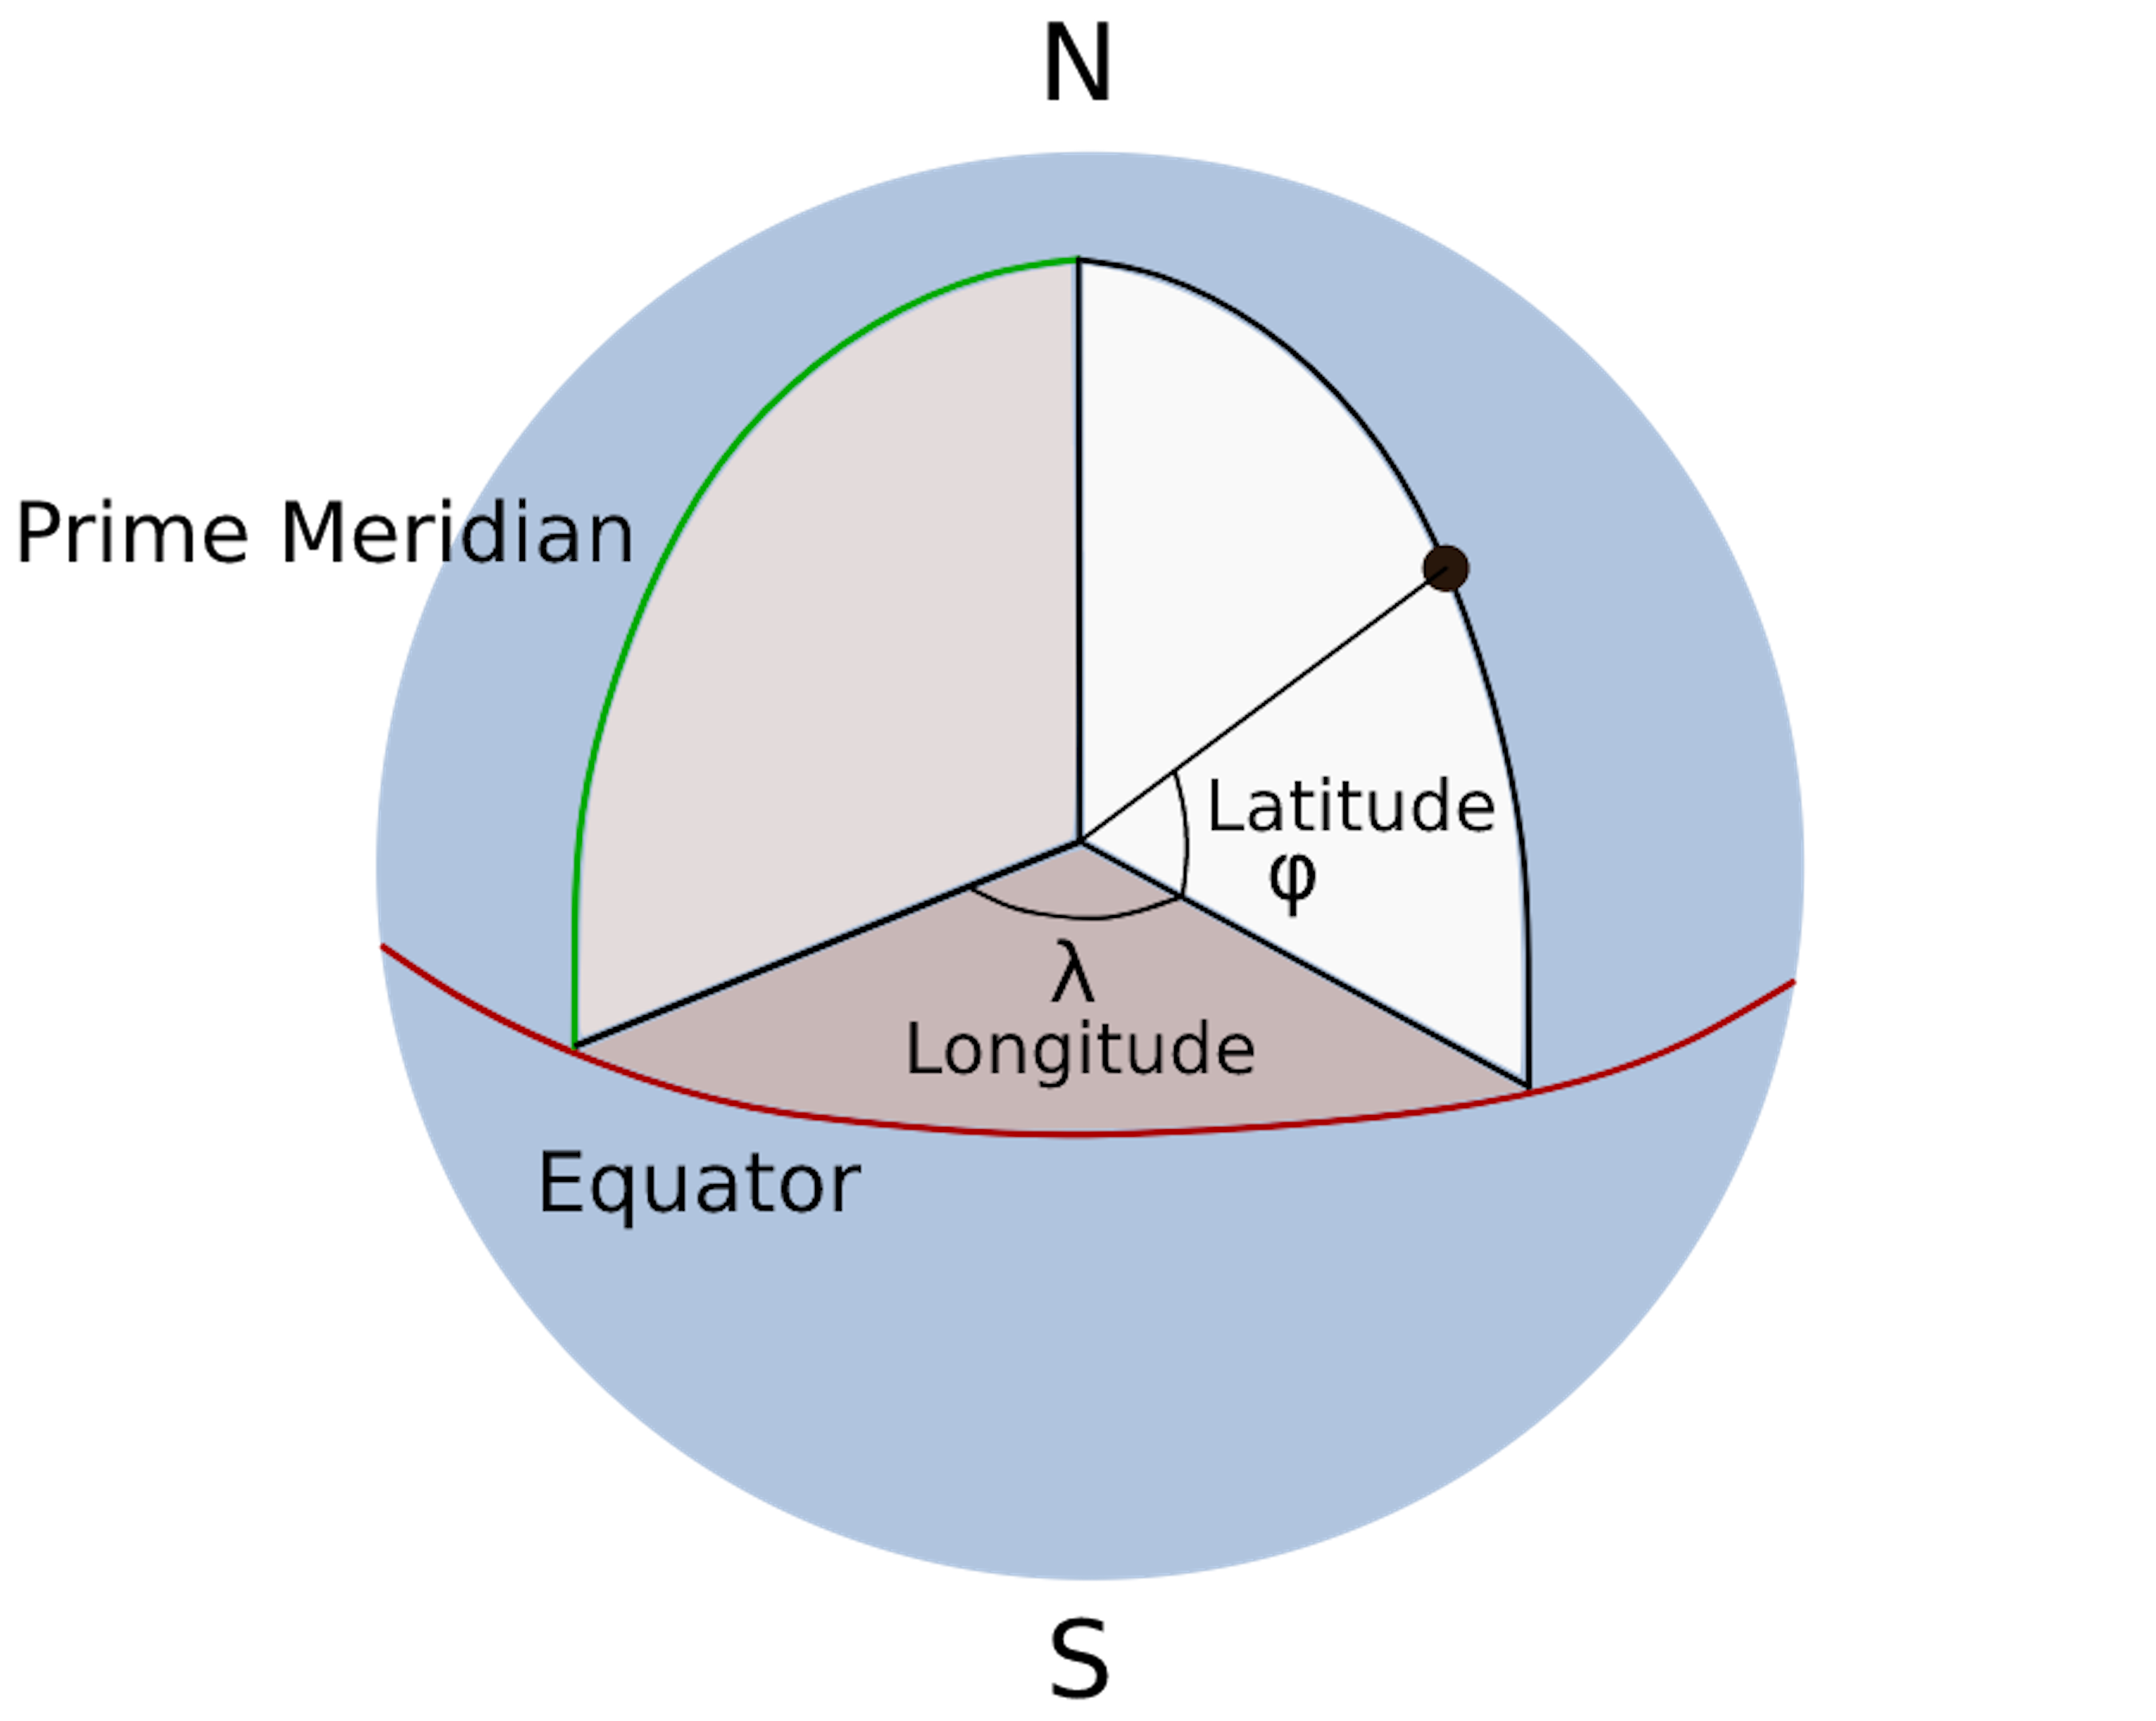
\includegraphics[width=0.9\textwidth]{Figures/latlong.png}
%   \caption[Illustration of latitude and longitude]{Illustration of the earth, and how latitudes and longitudes are calculated with respect to the equator and the prime meridian.}
%   \label{fig:latlong}
% \end{figure}


% \subsection{How to access tables and figures from the Simulation study}
% Here is a table for a single covariance level:
% % latex table generated in R 4.2.1 by xtable 1.8-4 package
% Thu Dec 14 12:52:54 2023
\begin{table}[ht]
\centering
\begin{tabular}{lrrr}
  \hline
Method & Mean & Quantile\_2.5 & Quantile\_97.5 \\ 
  \hline
Relaimpo & 0.125211 & 0.116182 & 0.133762 \\ 
  BVI & 0.125146 & 0.117180 & 0.133329 \\ 
  ELMG & 0.125138 & 0.117082 & 0.133092 \\ 
  ERW & 0.125130 & 0.117086 & 0.133242 \\ 
   \hline
\end{tabular}
\end{table}


% Here is one of the violin plots. The formatting of these might need som altering as it does not appear to nice right now. 
% \begin{figure}[ht]
%     \centering
%     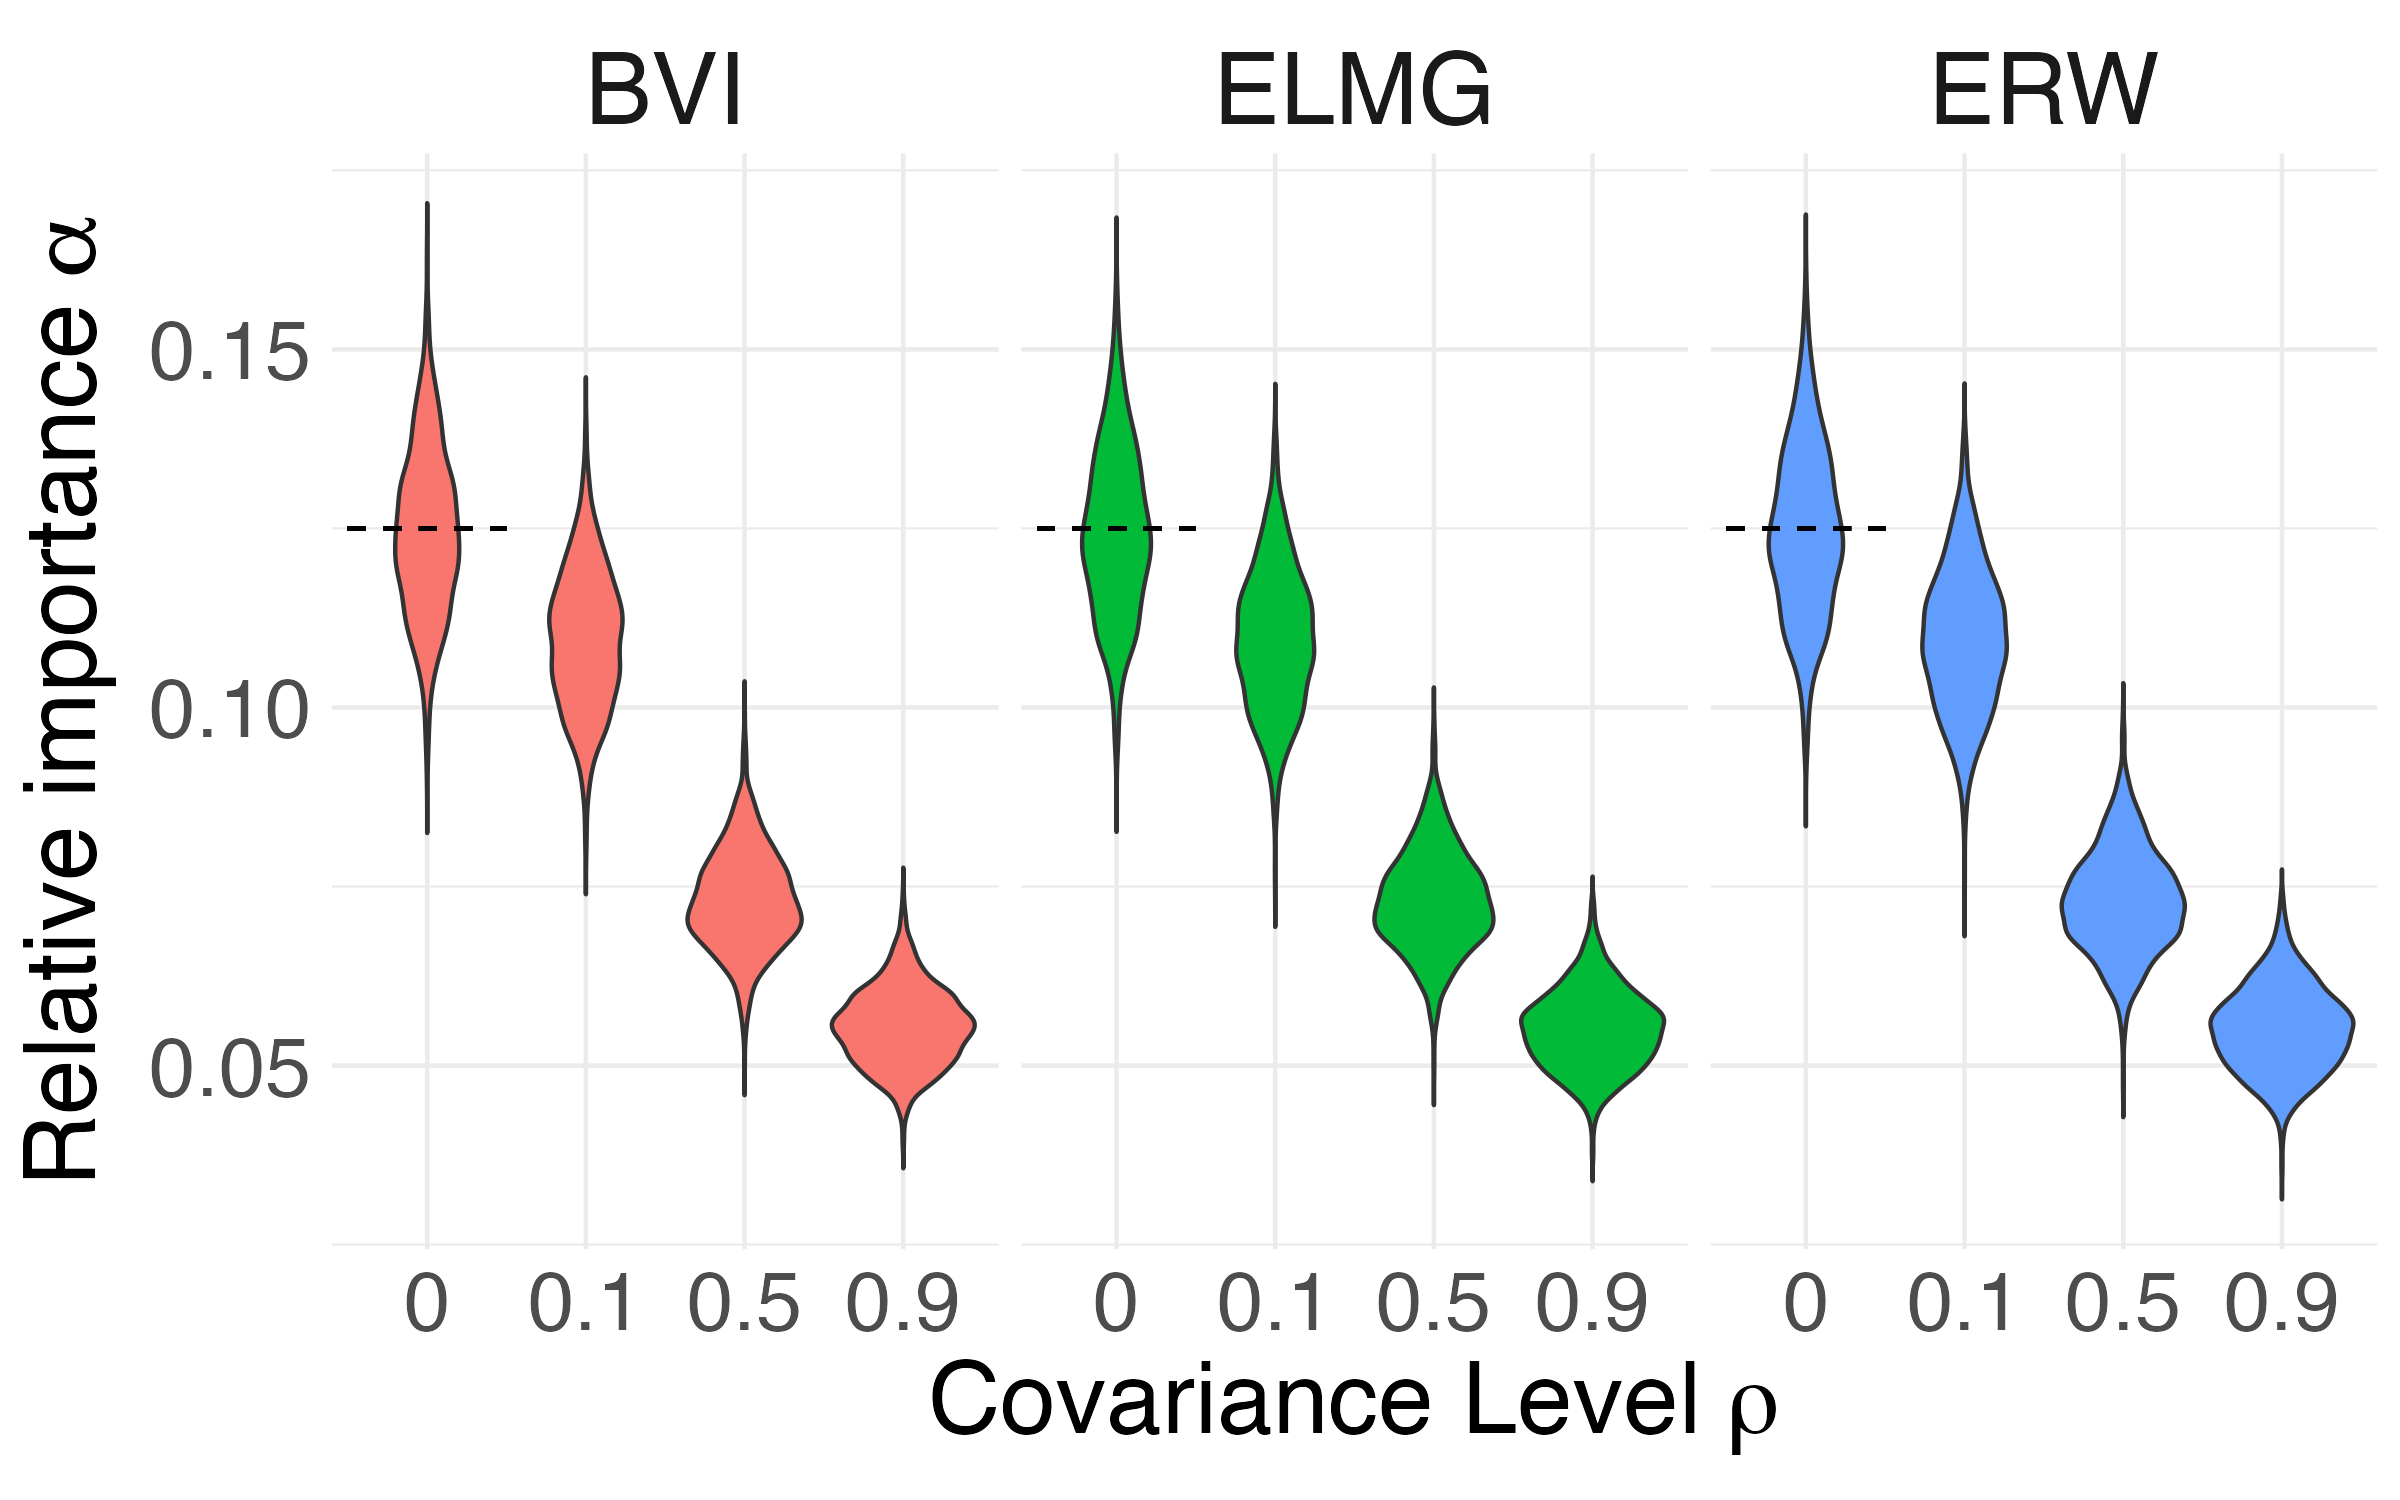
\includegraphics[width=\linewidth]{Figures/ViolinPlots/Variance_gamma.png}
%     \caption{Caption for the figure.}
%     \label{fig:my_label}
% \end{figure}



% \subsection{Citations}
% Here are some examples on how to reference a source (where none is relevant to the text but just for illustration purposes only). One may citet a single reference by calling \citet{wolves_of_mount_mckinley}, or several in the same bracket by calling \citet{machine_learning, clustering_impossibility} when they are all related to the same statement. There are many different styles on how to citet, and how the layout and order of your citation style is presented. This is my favorite, as I find it neat and tidy \citet{sheep}. It will show up in order of appearance in the references section.